\section{Laboratory work implementation}

\subsection{Tasks and Points}
\begin{enumerate}
	\item  Realizeaza un mini site cu 3 pagini statice
	\item  Site-ul trebuie sa pastreze toata informatia intr-o baza de date
	\item  Site-ul trebuie sa contina AJAX Requests.
	
\end{enumerate}

\subsection{Analiza lucrarii de laborator}

Click on \href{https://github.com/OctavianCoroletchiTI154/MIDPS.git}{"Link"} or copy \url{https://github.com/OctavianCoroletchiTI154/MIDPS.git} pentru repozitoriul meu.
\par Task a: \\
Dupa realizarea mockup-ului, am inceput sa contruiesc la inceput pagina de baza, Home Page. Dupa aia, formam link-urile spre paginile exterioare, cum ar fi register-page, contact-page, utilizatorul deja logat, si diverse pagini dinamice, care se incarca odata cu nevoia de anumite necesitati. Toate acestea au fost realizate cu ajutorul limbajelor HTML, care mi-a permis sa construiesc paginile propriu-zise. Cu ajutorul CSS(Cascadin Style Sheets), am personalizat toate micile detalii, culorile si marimile. Aceasta a oferit o vizualizare cit mai placuta. Cu ajutorul limbajulului PHP am facut conexiuni, cum ar fi cea cu baza de date.(->Vezi fig a-1,a-2,a-3). Intreaga structura a site-ului va folosi fisierele aratate in fig a-4.\\
\clearpage
\par Task b: \\
Pentru a depozita toata informatia, cum ar fi cea a logarilor utilizatorilor, sau a produselor soft deja introduse pe site, am avut nevoie de o baza de date. Personal, am stocat toata informatia pe un server, toata aceasta fiind editata in phpMyAdmin, cu ajutorul MySql(-> Vezi Fig b-1). MySql este un limbaj aparte, cu comenzile specifice, INSERT, UPDATE, CREATE s.a. Aici am stocat toata informatia tilizatorilor, precum parole, email-uri sau toate produsele introduse pe site.Utilizatorul poate introduce produse direct pe site, care mai apoi in urma unei conexiuni cu baza de date, se va introduce cu ajutorul unor comenzi. Aceasta va ramine acolo pina la urmatoare necesitate.\\
\par Task c:\\
Pentru a folosi interactionari directe cu serverul, am folosit AJAX(Asynchronous JavaScript And XML) Request. Aceasta ne permite sa face update la pagina fara a se face un refresh. Acesta interactioneaza cu serverul in spatele paginii web. AJAX Request permite unele posibilitati pentru care putem crea pagini user-friendly si usor de utilizat, fara incarcari ulterioare de pagini. Atunci cind se va tasta un buton, sau face click pe o anumita portiune, se va putea permite anumite schimbari realizate direct.(Vezi figurile c-1,c-2,c-3,c-4)\\

\subsection{Imagini}
\begin{center}
\vspace{30 mm}
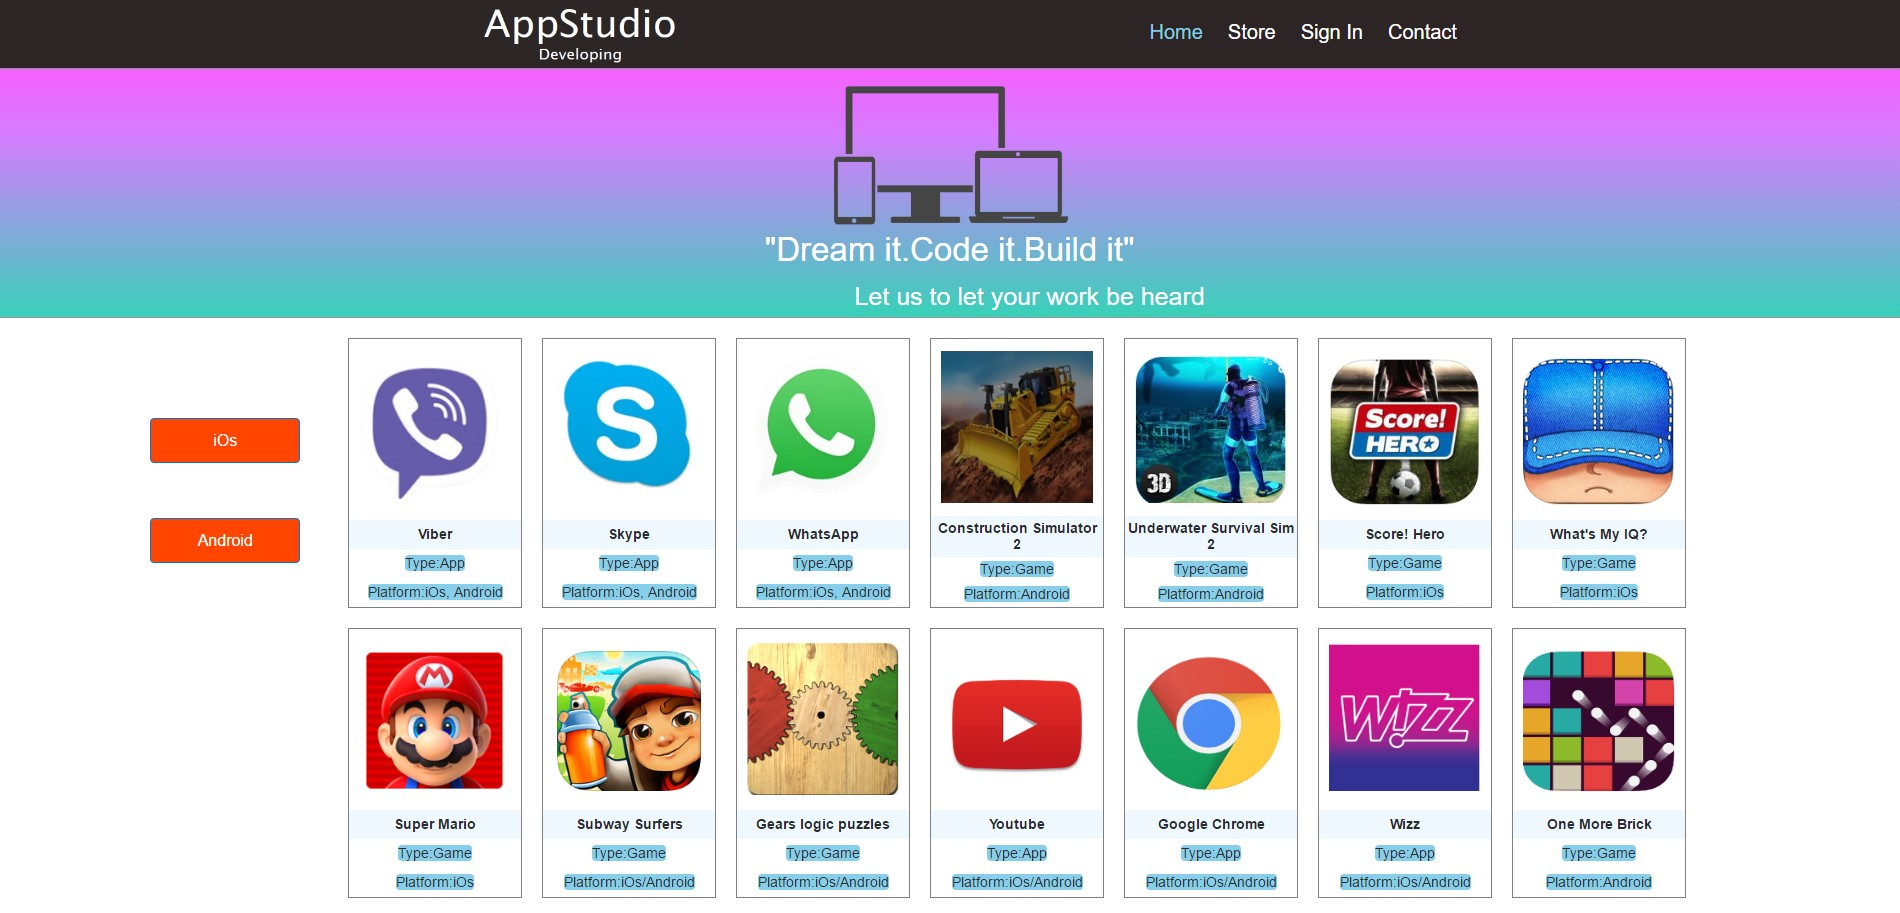
\includegraphics[scale=0.37]{1sthalfwebsite} \\ 
Fig a-1 - "Prima jumate a Home Page" \\
\vspace{10 mm}
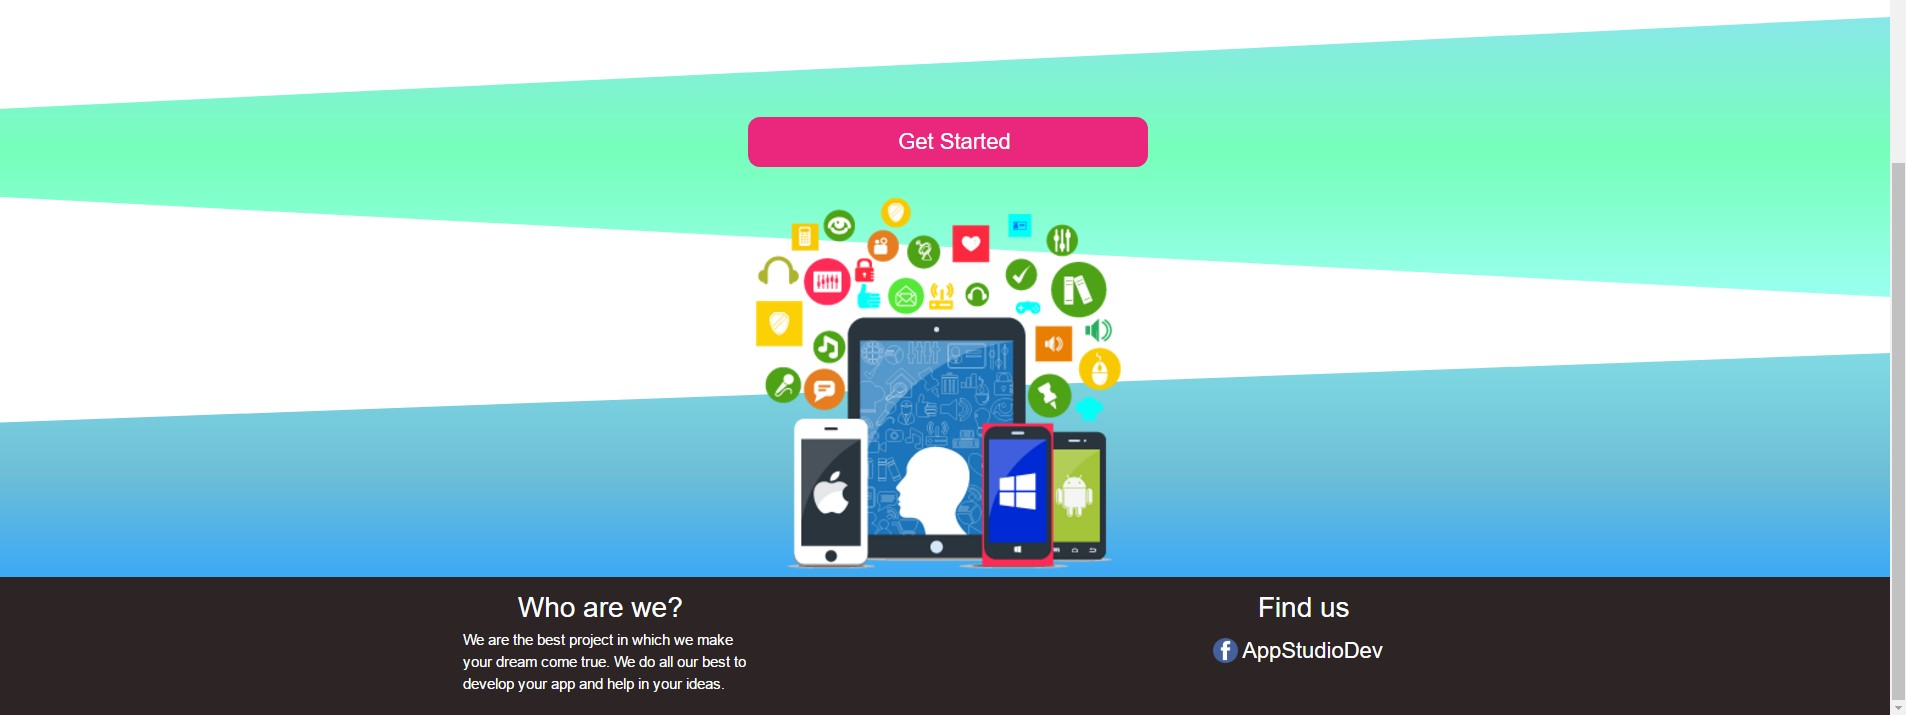
\includegraphics[scale=0.37]{2ndhalfwebsite} \\
Fig a-2- "A 2-a jumate a Home Page" \\
\vspace{10 mm}
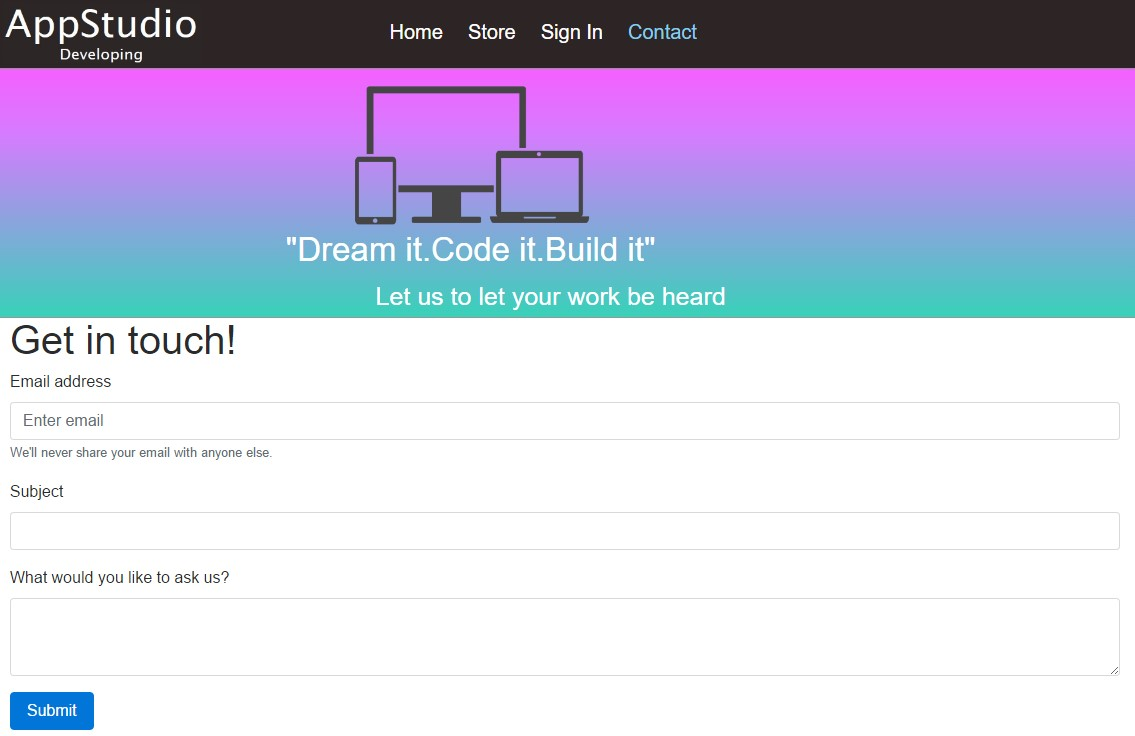
\includegraphics[scale=0.62]{contact} \\
Fig a-3 - "Pagina Contact" \\
\vspace{10 mm}
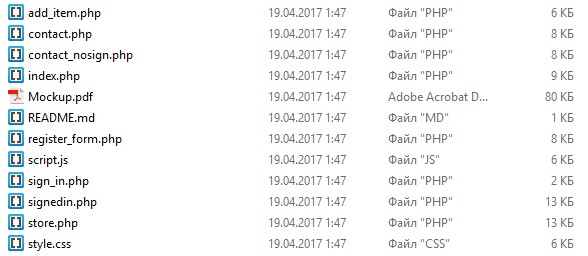
\includegraphics[scale=1]{used_files} \\
Fig a-4 - "Fisierele utilizate" \\
\vspace{10 mm}
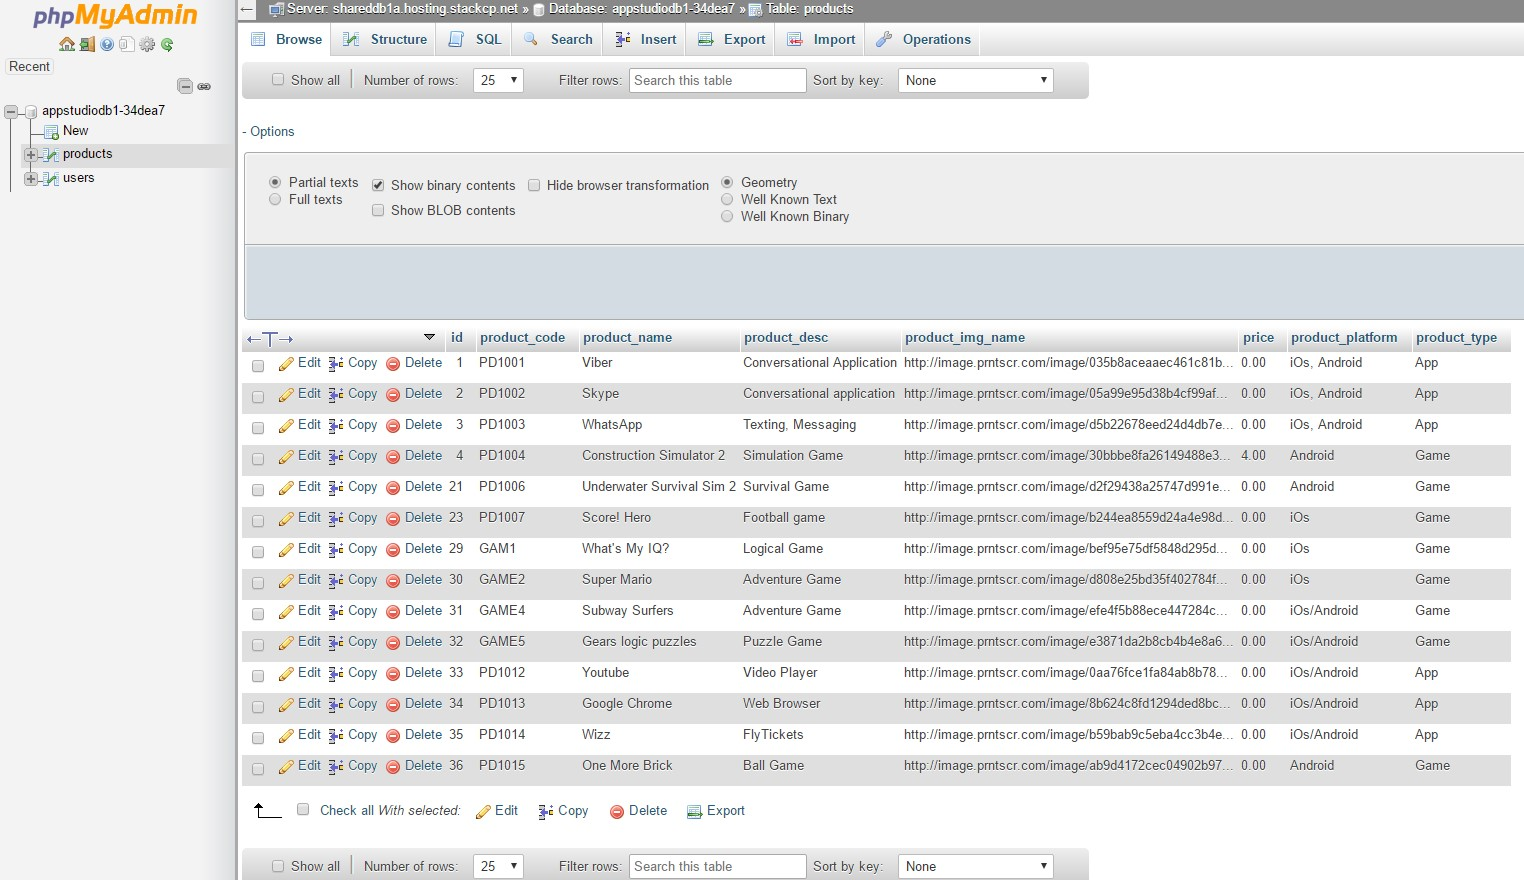
\includegraphics[scale=0.45]{phpMyAdmin} \\
Fig b-1 - "Infatisarea bazei de date print intermediul phpMyAdmin" \\
\vspace{10 mm}
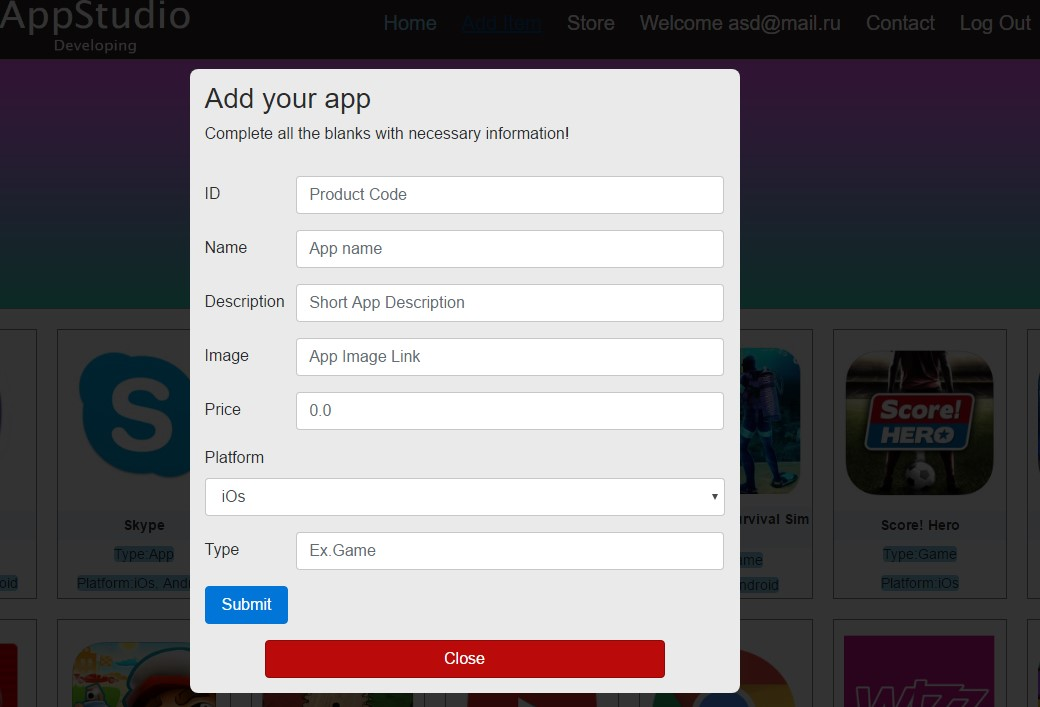
\includegraphics[scale=0.55]{addingitems} \\
Fig c-1 - "Adaugarea produselor cu ajutorul AJAX Request" \\
\vspace{10 mm}
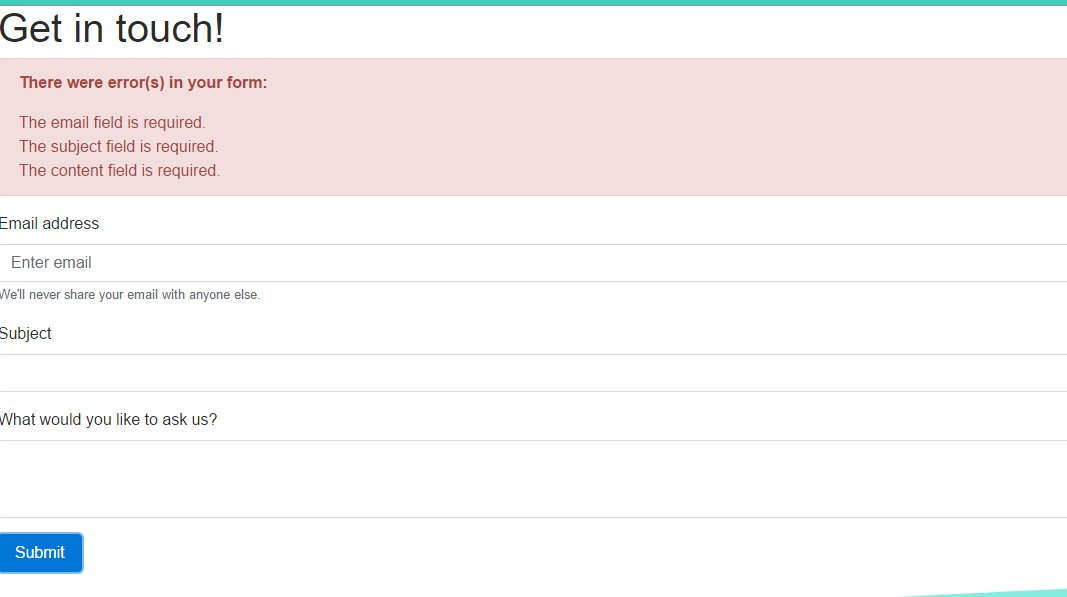
\includegraphics[scale=0.55]{contacterror} \\
Fig c-2 - "Afisarea erorilor cu ajutorul AJAX Request" \\
\vspace{10 mm}
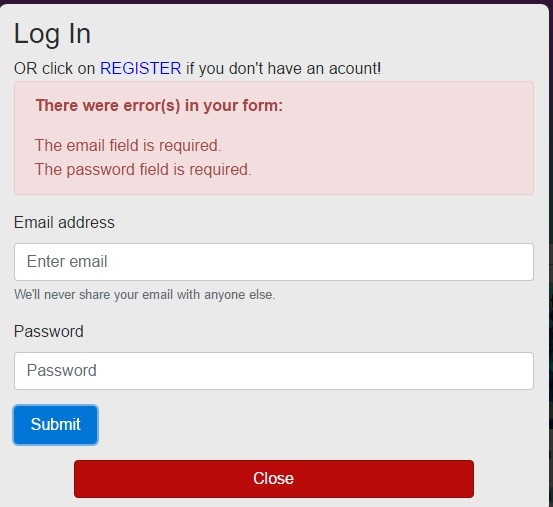
\includegraphics[scale=0.55]{errorlogin} \\
Fig c-3 - "Afisarea erorilor cu ajutorul AJAX Request" \\
\vspace{10 mm}
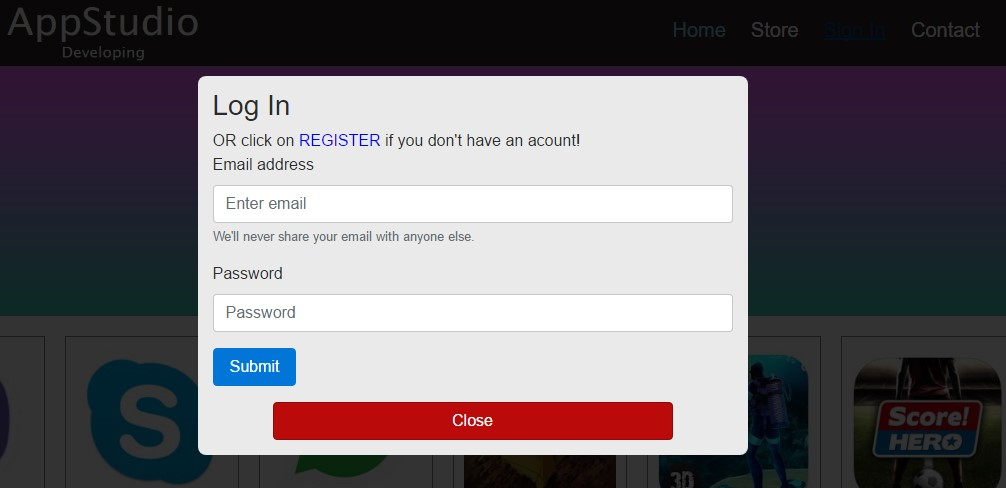
\includegraphics[scale=0.55]{signin} \\
Fig c-4 - "Logarea cu ajutorul AJAX Request" \\
\vspace{10 mm}



\end{center}


